\section{Laboratorial Testing} \label{sec:Lab}

In the laboratory, it was possible to simulate with real components the circuit in Figure \ref{fig:rc}. However, there were used some components that were not allowed for the theoretical and simulation analysis such as resistors with 2k$\Omega$ and more that three resistors of 1k$\Omega$. So the values used for the components were:
\begin{table}[!htb]
\centering
  \begin{tabular}{|c | c|}
    \hline    
\bf Component  & \bf Value\\ \hline 
R1  & 0.67 k$\Omega$ \\ \hline 
R2  & 1.00 k$\Omega$ \\ \hline 
R3  & 100.00 k$\Omega$ \\ \hline 
R4  & 0.50 k$\Omega$ \\ \hline 
C1  & 220.00 nF \\ \hline 
C2  & 220.0 0nF \\ \hline 

\end{tabular}
 \caption{Components used in the laboratory}\label{tab:labb}
\end{table}

With $R_2= 1k\Omega \parallelsum 1k\Omega$ and $R_4= 1k\Omega \parallelsum 2k\Omega$.

The results obtained were, for a frequency of $f = 1\ kHz$: 

\begin{align*}
  v_i &= 64.0\ mV \\
  v_o &= 5.9\ V \\
  Gain &\approx 90.68 \\
  Gain_{dB} &\approx 39,15 \\
\end{align*}

Altough we didn't use this exact values, the laboratory work helped to understand how the circuit work and the changes we will need to do, in the following analysis, to achieve the desired values.

\begin{figure}[h] \centering
  \begin{minipage}{.5\textwidth}
    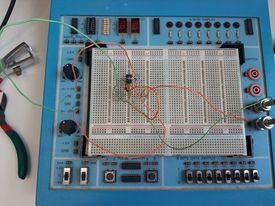
\includegraphics[width=.9\textwidth]{lab1.jpg}
    \caption{Image of the circuit built in the laboratory}
    \label{fig:simenv}
    \end{minipage}%
  \begin{minipage}{.5\textwidth}
  \centering
    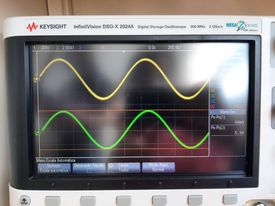
\includegraphics[width=.9\textwidth]{lab2.jpg}
    \caption{Results obtained in the osciloscope}
    \label{fig:compenv}
      \end{minipage}%
\end{figure}

\section{Theoretical Analysis} \label{sec:analysis}
 
The transfer function that caracterizes the studied circuit is given by

\begin{equation} \label{eq:transfer}
 \text{T(s)}=\frac{\text{R\textsubscript1}}{\text{Z\textsubscript{C1}+R\textsubscript1}} \left( 1+\frac{\text{R\textsubscript3}}{\text{R\textsubscript4}}\right) \frac{\text{Z\textsubscript{C2}}}{\text{Z\textsubscript{C2}+R\textsubscript2}}
\end{equation}

where Z\textsubscript{C1} and Z\textsubscript{C2} are the capacitor's impedances.

Analysing the present circuit, it's easy to understand that the term $ 1+\frac{\text{R\textsubscript3}}{\text{R\textsubscript4}}$ is proportional to the linear voltage gain, whereas R1 and C1 control the low cut-off frequency (f\textsubscript{L}) and R2 and C2 control the high cut-off frequency (f\textsubscript{H}).

The lower and upper cut-off frequencies correspond to the frequencies 3db bellow the maximum dB gain (\input{../mat/max.tex} dB). Then, the central frequency was computed by the geometric mean:

\begin{equation}
 \text{f\textsubscript{c}}= \sqrt{\text{f\textsubscript{L}} \times \text{f\textsubscript{H}}}
\end{equation}

The results are the following:

\begin{table}[!htb]
\centering
  \begin{tabular}{|c | c|}
    \hline    
    \input{../mat/frequencies.tex}
 \end{tabular}
 \caption{Central and cut-off frequencies}\label{tab:theo:frequencies}
\end{table}

The following graphics are obtained directly from the transfer function's (\ref{eq:transfer}) magnitude and argument, respectively:


\begin{figure}[h] \centering
  \begin{minipage}{.45\textwidth}
    \includegraphics[width=.8\textwidth]{T.eps}
    \caption{Frequecy response - Gain(dB)}\label{fig:theo:gain}
  \end{minipage}%
    \hspace{2 mm}
  \begin{minipage}{.45\textwidth}
  \centering
    \includegraphics[width=.8\textwidth]{Tphase.eps}
    \caption{Frequecy response - Phase (degrees)}\label{fig:theo:phase}
      \end{minipage}
\end{figure}

\subsection{Input and Output Impedances}

To compute the input and output impedances, we followed the ideal OP-AMP model : Z\textsubscript{in}=$\infty$ and Z\textsubscript{out}=0, resulting in the following equations:

\begin{gather}\label{impedances}
\begin{cases}
  |Z_i| = |Z_{C1} + R1 \parallelsum \infty| = |Z_{C1} + R_1|\\
  |Z_o| = |Z_{C2} \parallelsum (R_2 + R_3 \parallelsum 0)| = |Z_{C2} \parallelsum R2| 
  = |\frac{Z_{C2}R_2}{Z_{C2}+R_2}|\\
 \end{cases}
\end{gather}

 Considering that:
 
 \begin{gather}
 \begin{cases}
    v_- = v_+ = \frac{R1}{R1+Z_{C1}} v_i\\
    v_A = \left(1 + \frac{R3}{R4}\right) v_-\\
    v_o = \frac{Z_{C2}}{Z_{C2}+R2} v_A\\
  \end{cases}
\end{gather}
The results are the following:

\begin{table}[!htb]
\centering
  \begin{tabular}{|c|c|}
    \hline    
    \input{../mat/impedances.tex}
 \end{tabular}
 \caption{Real part of the input and output impedances}\label{tab:theo:impedances}
\end{table}

In the following table, there are the final result for the value of the merit, such as all the quantities that influence it (Gain obtainded, Gain Deviation, Central Frequency, Frequency Deviation and Cost):


\begin{table}[!htb]
\centering
  \begin{tabular}{|c | c|}
    \hline    
    \input{../mat/final.tex}
 \end{tabular}
 \caption{Central and cut-off frequencies}\label{tab:theo:frequencies}
\end{table}



% \subsection{Gain Stage}
% \subsubsection{Operating Point}
% The bias circuit V\textsubscript{cc}, R\textsubscript1, R\textsubscript2 will determine the base voltage V\textsubscript B and ensure the BEJ is on.
% 
% To be easier to analyse the bias circuit we can ignore the capacitors and make a Thévenin equivalent, replacing resistors R\textsubscript{1} and R\textsubscript{2}, which are in parallel, with an equivalent resistor R\textsubscript{B}:
% \begin{equation}
% R_B = \frac{R_{B1} R_{B2}}{R_{B1}+R_{B2}}
% \end{equation}
% 
% Looking at the circuit as a voltage divider, we have
% \begin{equation}
% V_{eq} = \frac{R_{B2}}{R_{B1}+R_{B2}} V_{cc}
% \end{equation}
% 
% To calculate the current passing through the node \textit{e} we know that I\textsubscript E =(1+$\beta_F$)I\textsubscript B.
% 
% Using the mesh analysis for the mesh on the left side and assuming that the current is going clockwise,
% \begin{equation}
% V_{eq} + R_B I_{B1} + V_{BEON} + R_{E1} I_{E1} = 0 \Leftrightarrow I_{B1} = \frac{V_{eq}-V_{BEON}}{R_B + (1+\beta_{FN}) R_{E1}}
% \end{equation}
% 
% From this transistor model, we also know that
% \begin{equation}
%  I_{C1}=\beta_{FN}*I_{B1};
% \end{equation}
% 
% \begin{equation}
%  I_{E1}=(1+\beta_{FN})*I_{B1};
% \end{equation}
% 
% \begin{equation}
%  V_{c}=V_{cc}-R_{c}I_{C1};
% \end{equation}
% 
% In the operating point calculations, we are also checking if the transistor is in the forward active region:  V\textsubscript{ce} = \input{../mat/FAR.tex} $>$ 0.7= V\textsubscript{BEon}, as we inteded.
% \subsubsection{Incremental Analysis}
% Following the operating point analysis, we can compute, the following incremental data, which concerns the bipolar transitor small signal model (AC)
% \begin{align*} 
% g_{m1}= I_{C1}/V_{T}\\
% r_{\pi 1}=\beta_{FN}/g_{m1}\\
% r_{o 1}=V_{AFN}/I_{C1}
% \end{align*}
% 
% where $g_{m1}$ is the transconductance, $V_{T}$=25mV is the termal voltage, $r_{\pi 1}$ is the input incremental impedance, $\beta_{FN}$=178.7 is the common emmiter current gain, $r_{o 1}$ is the output incremental resistance, and finally, $V_{AFN}$=69.7V is the forward mode early voltage.
% 
% 
% Assuming that the capacitor C\textsubscript{E} is a short-circuit when we are analysing the AC component, we have R\textsubscript{E}=0,
% 
% \begin{equation}
% \begin{cases} 
% \frac{vo}{vi}=-g_{m1} (R_C\parallel r_{o1}) \frac{r_{\pi1} \parallel R_B} {R_s+r_{\pi1}\parallel R_B} v_s \\
% Z_I= R_B \parallel r_{\pi1} \\
% Z_0=R_C\parallel r_{o1}
% \end{cases}
% \end{equation}
% 
% The results are shown in the following table.
% 
% \begin{table}[!htb]
% \centering
%   \begin{tabular}{|c|c|}
%     \hline    
%     {\bf Parameter} & {\bf Value} \\ \hline
%     \input{../mat/gainstage.tex}
%  \end{tabular}
%  \caption{Results Gain Stage}\label{tab:gainstage}
% \end{table}
% 
% As we can see, we are increasing the input voltage by 44 dB. The imput impedance is also pretty compatible with the resistance R\textsubscript S (Z\textsubscript I$>>$ ) R\textsubscript S. Unfortunately, Z\textsubscript O isn't compatible with the load impedance (8 Ohm), hence yhe inclusion of the output stage.
% 
% \subsection{Output Stage}
% 
% In this stage, we followed similar steps in order to compute the gain and impedances regarding this subcircuit.
% 
% Computing the operating point, we have
% 
% \begin{equation}
%  \begin{cases}
%   I_{E2}=\frac{V_{CC}-V_{EBON}-VI{2}}{R_O} \\
%   I_{C2}=\frac{\beta_{FP}}{\beta_{FP}+1}I_{E2}\\
%   V_{02}=V_{CC}-R_O I_{E2}
%  \end{cases}
% \end{equation}
% 
% Once again, we can compute, the following incremental data, which concerns the bipolar transitor small signal model (AC)
% \begin{equation}
%  \begin{cases}
% g_{m2}= I_{C2}/V_{T}\\
% r_{\pi 2}=\beta_{FP}/g_{m1}\\
% r_{o 2}=V_{AFP}/I_{C2}
%  \end{cases}
% \end{equation}
% 
% where $g_{m2}$ is the transconductance, $r_{\pi 2}$ is the input incremental impedance, $\beta_{FP}$=227.3 is the common emmiter current gain, $r_{o 1}$ is the output incremental resistance, and finally, $V_{AFP}$=37.2V is the forward mode early voltage.
% 
% Finally, we compute the output stage's gain and impedances:
% \begin{equation}
%  \begin{cases}
%  \frac{vo}{vi}=\frac{g_{m2}}{g_{\pi 2}+g_O+g_{o2}+g_{m2}}\\
%   Z_{I2}=\frac{g_{\pi 2}+g_O+g_{o2}+g_{m2}}{g_{\pi 2}(g_O+g_{o2}+g_{m2})}\\
%   Z_{02}=\frac{1}{g_{\pi 2}+g_O+g_{o2}+g_{m2}}
%  \end{cases}
% \end{equation}
% 
% where $g_{\pi 2}$ is the input incremental conductance, $g_{o 2}$ and $g_O$ is the $R_O$'s conductance
% 
% 
% The results are shown in the following table.
% 
% \begin{table}[!htb]
% \centering
%   \begin{tabular}{|c|c|}
%     \hline    
%     {\bf Parameter} & {\bf Value} \\ \hline
%     \input{../mat/outputstage.tex}
%  \end{tabular}
%  \caption{Results Output Stage}\label{tab:outputstage}
% \end{table}
% 
% As we can see, $Z_{I2}$ is very compatible with gain stage's output impedance ($Z_{I2}>>Z_{01}$), hence the two subcircuits can be connected without significant loss. Also, $Z_{O2}<<R_{load}$, hence there's less amplification loss.
% 
% 
% The theoretical operating point analysis is mostly in tune with the simulated result, for the gain stage only parameters there is a fine tune. Deviations start to occur when we compared values that are majorly influenced by the coupling of the two stages. But even then they are approximately equal.
% 
% \begin{table}[!htb]
%   \begin{minipage}{.5\linewidth}
%      \centering
%   \begin{tabular}{|c|c|}
%     \hline    
%     {\bf Parameter} & {\bf Value} \\ \hline
%     \input{../mat/OP.tex}
%  \end{tabular}
%  \caption{Results of theoretical analysis (operating point in volts)}
%  \label{tab:merit}
%   \end{minipage}%
%     \hspace{2 mm}
%     \begin{minipage}{.5\linewidth}
%       \centering
%         \begin{tabular}{|c|c|}
%     \hline    
%     {\bf Parameter} & {\bf Value} \\ \hline
%     @va[i] & 1.259429e+00\\ \hline
@hvc[i] & -1.33726e+00\\ \hline
@gib[i] & -1.20692e+00\\ \hline
@id[current] & 1.009703e+00\\ \hline
@r1[i] & -1.25943e+00\\ \hline
@r2[i] & -1.20692e+00\\ \hline
@r3[i] & -5.25053e-02\\ \hline
@r4[i] & 9.318730e-01\\ \hline
@r5[i] & 2.216626e+00\\ \hline
@r6[i] & -3.27556e-01\\ \hline
@r7[i] & -3.27556e-01\\ \hline
v(1) & 1.293920e+00\\ \hline
v(2) & 3.748740e+00\\ \hline
v(3) & 5.189374e+00\\ \hline
v(3b) & 5.189374e+00\\ \hline
v(4) & 1.458724e+00\\ \hline
v(5) & -5.34994e+00\\ \hline
v(6) & 4.516972e+00\\ \hline
v(7) & 4.185212e+00\\ \hline

%  \end{tabular}
%         \caption{Results of simulation analysis (operating point in volts)}
%         \label{compmerit}
%     \end{minipage} 
% \end{table}
% \newpage
% \subsection{Frequency Response}
%  In this subsection, we tried to study the circuit's response over different input frequencies. To achieve a better high cut off frequency, we considered a transistor incremental model with capacitance, as we can see in the picture bellow.
%  
%  \begin{figure}[h] \centering
% 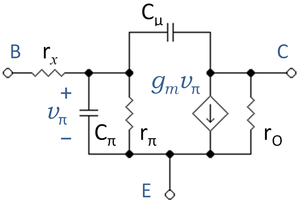
\includegraphics[width=0.4\linewidth]{transistor.png}
% \vspace{-3mm}
% \caption{Transistor incremental model with capacitance}\label{fig:rc}
% \end{figure}
% 
% The transistors' capacitances are conccuring with the spice model.
% 
% \begin{equation}
%  \begin{cases}
%   C_{\pi 1}=16.1pF\\
%   C_{\mu 1}=4.388pF\\
%   C_{\pi 2}=14pF\\
%   C_{\mu 2}=11.13pF
%  \end{cases}
% \end{equation}
% 
% where $C_{\pi}$ refers to the base-emitter junction capacitance and $C_{\mu}$ is the colector-base junction capacitance.
% 
% The results are the following, after loops of mesh analysis of the entire circuit:
% 
%  \begin{figure}[h] \centering
% \includegraphics[width=0.5\linewidth]{frequencyresponse.eps}
% \vspace{-5mm}
% \caption{Theoretical Frequency Response}\label{fig:rc}
% \end{figure}
% 
% 
% \newpage
